\documentclass[preprint,amsmath,amssymb,aps, prb,showkeys]{revtex4-1}
\usepackage{graphicx}% Include figure files
\usepackage{bm}% bold math
\usepackage{color}
\usepackage{tabularx}
\usepackage{fullpage,subfigure,float,psfrag,textcomp,gensymb,tikz,siunitx}
\usepackage{booktabs,multirow, dcolumn}% Align table columns on decimal point
\usepackage{xspace}
\usepackage[bookmarks=true,pdftoolbar=true]{hyperref}
\hypersetup{%
  pdftitle = {MAX Phases: Cluster expansion},
  pdfkeywords = {pdf, hyperref, bookmarks},
  pdfauthor = {Anjana Talapatra}}
 \usepackage[all]{hypcap} 

\def\etal{\mbox{\it et al.\ }} 
\newcommand{\eq}[1]{Eq.~\ref{#1}}
\newcommand{\fig}[1]{Fig.~\ref{#1}}
\newcommand{\tab}[1]{TABLE~\ref{#1}}

\begin{document}

	%\preprint{APS/123-QED}

	\title{A high throughput combinatorial study of the effect of M site alloying on the solid solution behavior of M\texorpdfstring{$_2$}{}AlC MAX phases}
	\author{Anjana Talapatra$^{1}$}
	\email{anjanatalapatra@tamu.edu}
	\author{T. Duong$^{1}$}
	\author{W. Son$^{1}$}
	\author{H. Gao$^{1}$}
	\author{M. Radovic$^{1,2}$}
	\author{R. Arr\'{o}yave $^{1,2}$}
	\affiliation{$^{1}$ Department of  Materials Science \& Engineering, TAMU, USA, 77843}
	\affiliation{ $^{2}$ Department of Mechanical Engineering, TAMU, USA, 77843}
	\date{\today}

	\begin{abstract}
		In this work, a systematic investigation of the alloying behavior on the M sub-lattice of M$_2$AlC, where M is Ti,V,Zr and Hf with elements in the first transition metal row as well as Ca and Sc is carried out via a combination of alloy theoretic approaches and Density Functional Theory for 41 alloy systems. The cluster expansion formalism is used to explore the configurational space in ternary MAX phases. On the basis of their solid-solution behavior, the alloys are classified into three regimes: phase separation, weak ordering and strong ordering. Observed trends are investigated in terms of indicators at the electronic and structural levels. For the systems showing ordering, the ordered structures are identified and their structural 
and electronic properties are investigated. The likelihood of some of the systems to exist as solid solutions at finite temperature is discussed.
	\end{abstract}

	\keywords{MAX phases, Solid-solutions, DFT ,cluster expansion}

	\maketitle

%------------------------------------------------------------------------------------------------------------------------------------%
\section{Introduction}
\label{sec:Intro}
M$_{n+1}$AX$_n$ phases are layered ternary compounds that share many properties with ceramic and metallic materials alike~\cite{barsoum2013max, radovic2013max, barsoum2000, barsoum2004,barsoum2011elastic,sun2011progress}. Like metals, MAX phases tend to be relatively soft and readily machinable, with good thermal shock resistance as well as damage tolerance, in addition to being excellent thermal and electrical conductors. On the other hand, MAX phases as carbides and nitrides are similar to prototypical ceramics as they are refractory and thermodynamically stable up to elevated temperatures, resistant to chemical attack and have relatively low thermal expansion coefficients. In addition, some of them are oxidation, creep and fatigue resistant~\cite{radovic2013max}. Their properties are even more remarkable when one considers that at room temperature some MAX phases can be compressed to stresses over 1 GPa, achieving full recovery upon unloading, while dissipating 25\% of the mechanical energy do to reversible dislocation motion~\cite{
barsoum2003fully}. At higher temperatures, however, MAX phases undergo a brittle-to-plastic transition (BTPT)~\cite{benitez2016room} and can be plastically deformed for more than 25\% before failure even under tension~\cite{radovic2002effect}. Finally, they can be fabricated inexpensively using a variety of reaction sintering methods~\cite{sun2011progress,wang2010layered,barsoum2013max}. Given their remarkable mechanical properties,oxidation resistance and thermal stability, it is not surprising that MAX phases were first targeted for structural and multi-functional high-temperature applications. 

\begin{figure}
\centering
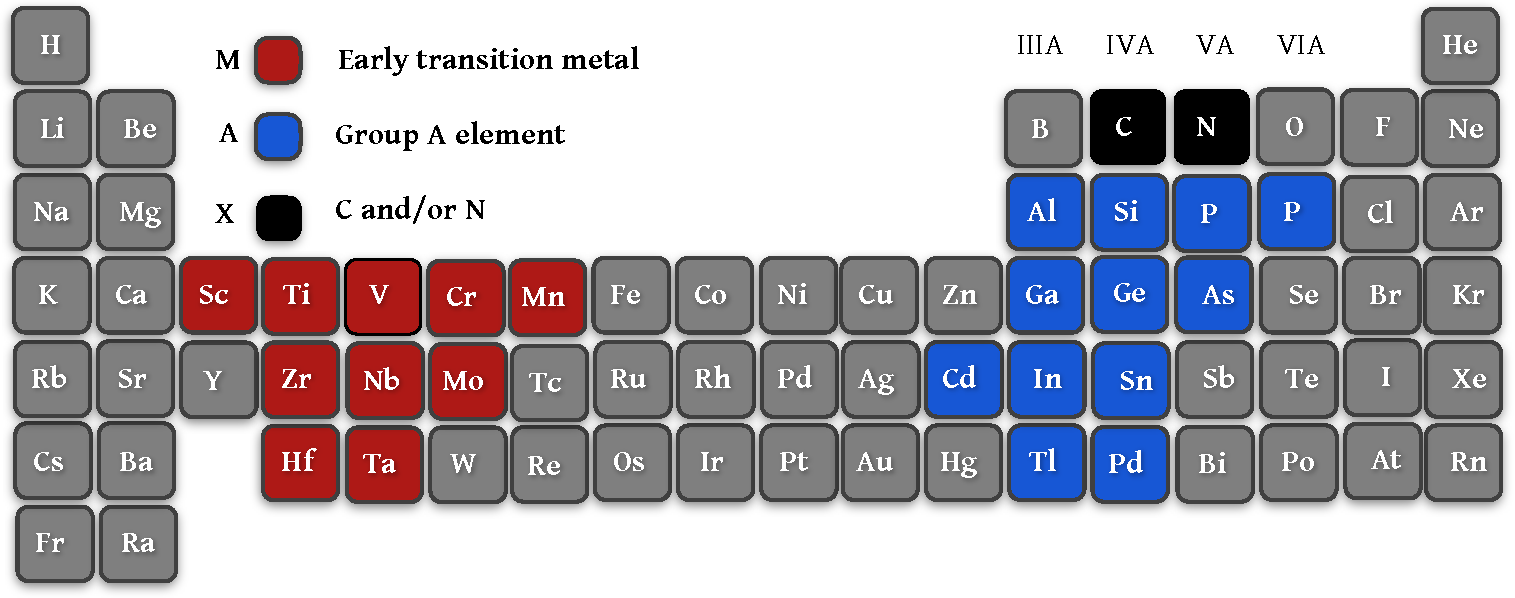
\includegraphics[width=0.95\textwidth]{figure_1}
\caption{Elements of periodic table which are known to form pure MAX phases.}
\label{fig:MAX_periodic_table}
\end{figure}

Despite the significant progress in understanding the composition-structure-properties relationship in MAX phases, only a small fraction of these compounds has been characterized to date, with even a smaller fraction of those characterized at elevated temperatures. While approximately 70 pure MAX phases have been synthesized and characterized~\cite{barsoum2010max}, the number of possible MAX phases is considerably larger when taking into account the distinct occupancies in the M, A and X sub-lattices as well as the possible layering sequences (i.e. 211, 312, 413, etc.). In fact, recently, DFT calculations have suggested that close to 600 MAX phase compositions are at least thermodynamically---that work neglected to consider possible competitions between the studied compounds and other competing phases originating from the binary subsystems---and mechanically stable~\cite{aryal2014genomic}. 

While hundreds of compounds may seem like a rather large chemical space, the number of possible stable MAX phases grows geometrically when one considers possible alloying substitutions in the M, A and/or X sub-lattices. Billions of combinations are possible ($\frac{600!}{598!2!}$) MAX phase pairs, with 10 composition intervals within each pseudo-binary amounts to 1.8$\times10^6$ possible compositions), without considering simultaneous alloying in more than one sub-lattice, e.g. (M$_1$,M$_2$)$_{n+1}$(A$_1$,A$_2$)(C,N)$_n$. Of this rather larger number of MAX solid solutions, less than a hundred have been synthesized and characterized~\cite{naguib2014new}. 

Mixing in the M, A or X sub-lattices has important consequences: For example, the additional configurational entropy:
\begin{equation}
 S\approx n^{*} k_B \left[ y^{} \ln\left(y^{}\right) + \left(1-y\right)\ln\left(1-y\right) \right] = \frac{\text{J}}{\text{mole-f.u. K}}
 \label{eq:mixing}
\end{equation}

\noindent where the pre-factor $n^*$ is substituted by $n+1$, $1$ or $n$ depending on whether substitution happens in the M, A or X sub-lattice) may contribute to the greater stability of MAX solid solutions, even in cases when the end-members are metastable~\cite{zhou2008new}. Mixing in solid solutions can result in significant improvements in compressive strength (e.g. (Ti$_{1-x}$V$_x$)$_2$AlC~\cite{meng2005strengthening} and (Ti$_{2}$)$_2$AlC$_{1-x}$N$_x$~\cite{barsoum2000processing}), although in other cases, such solid solution strengthening is not observed~\cite{salama2002synthesis,ganguly2004synthesis}. The possibility of synthesizing solid solutions also offers the opportunity of tuning some of the thermo-mechanical properties of MAX phases. For example, it has been demonstrated that in Cr$_2$(Al$_{x}$,Ge$_{1-x}$)C solid solutions, it is possible to achieve nearly isotropic thermal expansion---thermal expansion anisotropy tends to be the rule rather than the exception in pure MAX phases---at $x=0.75$~\cite{cabioch2013tailoring}. Finally, alloying may have dramatic effects on the magnetic 
properties of MAX solutions~\cite{mockute2013synthesis}. This is particularly true in the case of solid solutions involving mixing in the M sub-lattice with Mn being one of the constituents of the solid solution, as in (Cr$_{x},Mn$)$_2$AlC~\cite{dahlqvist2011magnetic}, due to the rather complex nature of Mn magnetic self-interactions~\cite{sandratskii2002exchange,larson1988theory}. 

Unfortunately, the opportunity to further tune/tailor the properties of MAX phases through alloying comes with a very steep price tag, as the size and dimensionality of the space to be explored in search of novel and practically relevant properties has exploded beyond current synthesis capabilities. In fact, the 100 or so MAX solid solutions discovered to date constitute an insignificant fraction of the entire MAX chemical space. Systematic exploration of all the possible combinations within the M, A or X sub-lattices in all layering sequences---the fact that end members with a particular stoichiometry have not been observed does not preclude the stability of the corresponding solid solutions---through conventional synthesis and characterization methods is beyond current capabilities. While high-throughput DFT calculations~\cite{saal2013materials,curtarolo2012aflowlib} may seem promising, when one compares the size of current repositories (about one million compounds over a couple of years) to the size of the chemical space to be explored (billions of possible combinations), it is clear that computational exploration of the MAX solid solution space is still daunting.   

The organization of this article is as follows: In section \ref{sec:prior}, we discuss the status quo in the area of MAX phase solid solutions in the context of prior experimental and computational work. In section \ref{sec:methods}, we describe the various approaches that will be applied in exploring the effect of configurational degrees of freedom on the thermodynamics in this work and the computational parameters used.In section \ref{sec:results} we present the results obtained and analyze the stability and electronic structure of the isolated phases. In section \ref{sec:discussion}, we discuss the physics underlying the results and seek to explain the trends observed. Finally, section \ref{sec:conclusion} includes a summary of the results and discusses future prospects in the light of conclusions drawn on the basis of this work.
%------------------------------------------------------------------------------------------------------------------------------------%
\section{Prior Experimental and Computational Work}
\label{sec:prior}

As mentioned above, to date, less than a hundred MAX solid solutions have been synthesized and characterized. Out of all known solid solutions, the most common stacking sequence corresponds to \textbf{211}, followed by the \textbf{312} and \textbf{413}~\cite{naguib2014new}. Due to their oxidation resistance~\cite{sundberg2004alumina, tallman2013critical, basu2011long} and their oxidation-induced crack healing properties~\cite{song2008oxidation,li2012multiple, sloof2016repeated}, aluminum-containing MAX phases are some of the most studied compounds in the MAX class and it is thus not surprising that the vast majority of the  MAX solid solutions are variants of (M$_1$,M$_2$)$_{n+1}$(Al,A$_2$)(C,N)$_n$. In this section, we will focus our discussion on some of the already experimentally verified \textbf{211} MAX solid solutions, with emphasis on those exhibiting mixing in the M sub-lattice. More details on other MAX solid solution systems can be found in Ref.~\cite{naguib2014new}.

One of the oldest investigation into solid solution behavior in MAX phases is the work by Schuster \etal~\cite{schuster1980ternary}. In that work, the Cr$_2$AlC, V$_2$AlC and Ti$_2$AlC systems as well as quaternary extensions were investigated through synthesis and XRD, after annealing at 1000$^o$C for 170 h. In the case of the Ti$_2$AlC-V$_2$AlC pseudo-binary, complete solid solution was observed, with lattice parameters varying almost in perfect agreement with Vegard's Law, although with a \emph{slight} negative deviation, suggesting a slight tendency for (short-range) ordering.  These results were later corroborated by Meng \etal~\cite{meng2005strengthening}, who also found that V had a strengthening effect on (Ti,V)$_2$AlC solid solutions, particularly due to the strengthening of M-Al bonds through the addition of extra valence electrons in the d channel from V~\cite{wang2004ab}. Schuster also investigated the (Cr,V)$_2$AlC system and found solubility across the entire composition range, with further 
corroboration by Yeh \etal~\cite{yeh2013formation} and Tian \etal~\cite{tian2009synthesis}. In this system, however, longer annealing times were necessary to reach equilibrium~\cite{schuster1980ternary}. Contrary to the (Ti,V)$_2$AlC and (Cr,V)$_2$AlC cases, no solid solution was observed in the Cr$_2$AlC-Ti$_2$AlC system~\cite{schuster1980ternary} except for some limited solubility close to the end members, mostly due to entropic effects.

Nowotny \etal~\cite{nowotny1982structural} reported MAX solid solutions with the compositions (Ti$_{0.5}$Nb$_{0.5}$)$_2$AlC, (Ti$_{0.4}$Ta$_{0.6}$)$_2$AlC,  (V$_{0.65}$Ta$_{0.35}$)$_2$AlC, (V$_{0.5}$Nb$_{0.5}$)$_2$AlC, (Nb$_{0.6}$Zr$_{0.4}$)$_2$AlC and (Nb$_{0.8}$Zr$_{0.2}$)$_2$AlC, although it was not reported in any of those cases whether there was an extensive range of solubility or whether these MAX solid solutions existed in equilibrium with other phases. Very recently, Naguib \etal~\cite{naguib2014new} revisited the case of (Nb$_{0.8}$Zr$_{0.2}$)$_2$AlC and confirmed a phase with the same stoichiometry that was at equilibrium with the Zr$_5$Al$_3$ and ZrC phases. Since this is a quaternary system (Nb-Zr-Al-C) the three-phase equilibrium is not invariant in composition and other solid solutions (Nb$_{x}$Zr$_{1-x}$)$_2$AlC may also be possible to synthesize. This, however, points to the difficulty in the characterization of MAX solid solutions, as competition with phases originating in the 
binaries (and even ternaries) must be taken into account~\cite{dahlqvist2010stability}.

Additional MAX solid solutions on M site with In as the A element have been investigated by Gupta \etal~\cite{gupta2006synthesis} and Barsoum \etal~\cite{barsoum2002fabrication}. Barsoum \etal report on the synthesis of (Ti$_{0.5}$Hf$_{0.5}$)$_2$InC solid solutions. Through XRD they were able to determine that the  (Ti,Hf)$_2$InC were indeed solid solutions as the measured lattice parameters corresponded to intermediate values of the end-members. Similarly, Gupta \etal reported the synthesis of (Ti$_{0.5}$Hf$_{0.5}$)$_2$InC solid solutions, although impurities (below 2\% vol.) of TiC$_x$ and ZrC$_x$ were present in the synthesized materials. Phatak \etal~\cite{phatak2009synthesis} reported the synthesis of (Cr$_{0.5}$V$_{0.5}$)$_2$GeC. The results indicated a decrease in the c-lattice parameter relative to the end-members.

Perhaps some of the most interesting recently discovered MAX solid solutions with 211 stacking correspond to those involving alloying of Mn in the M sub-lattice of Cr$_2$AC-based compounds. Dahlqvist \etal~\cite{dahlqvist2011magnetic} used DFT methods to investigate the ground state in (Cr$_{1-x}$, Mn$_x$)$_2$AlC alloys and found that the M site tended to undergo an ordering transition whereby FM-ordered Mn layers were coupled (via exchange) to nonmagnetic Cr layers. Furthermore, they predicted that by manipulating the degree of disorder between the Cr and M atoms in the M sub-lattice they could tune the magnetic coupling strength and sign. Mockute \etal~\cite{mockute2013synthesis} were then able to synthesize the compounds in the thin film state. They also presented an ab initio theoretical analysis of the temperature-dependent stability of of the solid solutions by computing the formation enthalpies relative to the most stable competing phases identified ( Cr$_2$AlC, Mn$_3$AlC, MnAl, and C) ~\cite{dahlqvist2011magnetic}. Their results show that the compounds are energetically stable over the composition range x = 0.0 to 0.5 for temperatures $>$ 600 K. 

Horlait \etal~\cite{horlait2016synthesis} employed experiments and density functional theory calculations in parallel to study the Zr$_2$(Al$_{1−x}$Bi$_x$)C (0 $\leq$ x $\geq$ 1) system. They showed that  the Zr$_2$(Al$_{0.42}$Bi$_{0.58}$)C MAX phase can be stabilized from powders even though the end members Zr$_2$BiC and Zr$_2$AlC are known to be unstable. Multiple random 128 atom supercells were used for the calculations.
Recently, Anasori \etal~\cite{anasori2015experimental} reported the discovery of two new ordered quaternary MAX phases - Mo$_2$TiAlC$_2$ and Mo$_2$Ti$_2$AlC$_3$. They showed that the  high energy penalty due to C surrounding the M atoms in a face-centered configuration drives the M layer ordering. The ordered structures also showed higher Young's moduli than the ternary end members. Special quasi-random structure (SQS) were used to model full or partial solid solutions on the M-sites. 

A theoretical investigation was carried out by Du ~\cite{du2009theoretical} approximated the Ti$_2$AlC$_{0.5}$N$_{0.5}$ solution by assuming a mixed occupancy (C and N) in the X sub-lattice of a Ti$_2$AlX structure. In their work on the Ti$_2$Al(C,N) solid solutions, Arroyave and Radovic~\cite{arroyave2011MAX} used the cluster expansion (CE) formulation~\cite{domb2000phase,de1994solid} to explore the energetics of C-N interactions across the entire Ti$_2$AlC-Ti$_2$AlN composition range. They showed that there exists a definite tendency for ordering in the (C,N) sub-lattice, however the C-N interactions are weak and the solution becomes disordered at relatively low temperatures. 
%------------------------------------------------------------------------------------------------------------------------------------%
\section{Methods}
\label{sec:methods}

\subsection{Approaches to Modeling Configurational Disorder}

One of the most direct approaches to investigate configurational effects on alloys is to simply use large (periodic) cells in which configurational disorder is simulated through the random decoration of sites. Electronic structure methods~\cite{kohn1965self,vasp} can then be used to calculate the properties of the resulting structures. Since cells are finite, the resulting configurations are not strictly random, although if the cell is large enough one could expect that the ensemble of local atomic environments would approximate that of a \emph{true} random alloy \emph{up to a certain distance}~\cite{wei1990electronic}. Multiple equivalent configurations can then be analyzed in order to obtain proper statistics. The ability of such an ensemble of local environments to reproduce the behavior of a true random solid solution depends on the property to be calculated---some properties of random alloys cannot be calculated from periodic cells even in principle---as well 
as the rate of decay of interatomic interactions.

Instead of performing statistical averages of 'random-like' configurations, approaches based on perturbation theory perform the configurational 'averaging' analytically~\cite{turchi2007interface}. A popular mean-field approach to configurational disorder is the Coherent Potential Approximation  (CPA)~\cite{yonezawa1973coherent}, and its variants. In the CPA, the random alloy is modeled  as an ordered lattice of 'effective atoms'. The coherent potential describing this effective medium is constructed by requiring that the electron scattering off the real atoms embedded in this mean field vanish on average. 

Yet another approach to simulate random solid solutions is to employ Special Quasirandom Structures (SQS)~\cite{zunger1990special}. SQS are small, \emph{periodic} supercells that are \emph{specially designed} to reproduce approximately the configurational structure of an infinite random alloy. The configurational state of a random alloy with a given underlying lattice and composition $x$ can be characterized by its many-body correlation functions~\cite{zunger1990special}. Rigorously, the ensemble average of a physical property can be 
expressed in terms of these correlation functions. In their 2010 work, Mockute \etal~\cite{mockute2015solid} used SQS to simulate the (Cr$_{1-x}$Mn$_x$)$_2$AlC solid solution.

All prior work on solid solutions focuses on an ad-hoc approach: investigating few compositions experimentally/computationally. First-principle calculations are essential in this regard. The prevalent methods are the use of SQS and supercells which have their own limitations. Using a 128 atom supercell, if we want to simulate ordering in the M site of a 211 MAX phase (M1$_{1-x}$M2$_x$)$_2$AX, we have 64 M sites. In theory, this means that to explore the ordering tendencies of the solid solutions we need to calculate a comprehensive number of ordered structures for each solid solution composition combination (i.e. each value of x). Computationally, this is prohibitively expensive. Hence the need for the Cluster expansion method.

\subsection{Cluster Expansion}
When the focus is on the energetics of an alloy, we can use yet another approach to investigate the effects of configurational degrees of freedom on the thermodynamic properties of an alloy. A cluster expansion (CE) is simply a compact representation of the energetics of an alloy in terms of collections of 'clusters' of lattice sites. Formally, a CE is defined by assigning occupation variables, $\sigma_i$ to each site $i$ of a lattice that has configurational degrees of freedom (i.e. an M site in a M$_2$AX lattice). The occupation variables are assigned specific values ($\pm1$ in a binary system) depending on the identity of the atom occupying the site. A particular arrangement of these 'spins' corresponds to a configuration which is then represented as a vector $\overline{\sigma}$ of spins $\sigma_i$. The CE then parametrizes the energy (or any other property) of the alloy in terms of the so-called correlation functions of the occupation variables:

\begin{equation}
E\left( \sigma  \right) = \sum\limits_\alpha  {{m_\alpha }{J_\alpha }\left\langle {\mathop \prod \limits_{i \in \alpha '} {\sigma _i}} \right\rangle }
\label{eq:ce}
\end{equation}

\noindent where $\alpha$ is a cluster (a collection of sites $i$). The sum is taken over all clusters $\alpha$ which are not equivalent by a symmetry operation of the space group of the lattice and the average is taken over all $\alpha '$ symmetry-equivalent clusters. The coefficients $J_{\alpha}$ are called the effective cluster interactions (ECIs) and relate a given configurational state to a particular energy. The multiplicities $m_{\alpha}$ correspond to the number of equivalent clusters (by symmetry) in a given configuration. The ECIs are obtained through the solution of an overdetermined algebraic problem where the (known, calculated) energy of a set of compounds is expressed as functions of the (known) correlation functions and the (unknown) ECIs for every symmetry-unique cluster considered. Solving for the unknown ECIs can be done through different approaches, including genetic algorithms~\cite{blum2005using}, compressive sensing~\cite{nelson2013compressive} as well as the conventional so-called structure 
inversion method~\cite{vanderwalleATAT,connolly1983density}. Once the cluster expansion is found---the convergence of the expansion is highly system-dependent---the energy of \emph{any} configuration can be calculated by simply applying ~\ref{eq:ce}. In this work, we will use the Cluster expansion method to explore the configurational space occupied by the (M1$_x$,M2$_{1-x}$)$_2$AlC solid solutions.

\subsection{Calculation Parameters}
The total energy calculations were performed within the density functional theory (DFT)~\cite{kohn1965self} framework, as implemented in the Vienna ab initio simulation package (VASP)~\cite{vasp,vasp2}. The generalized gradient approximation (GGA)~\cite{GGA} is used in the form
of the parameterization proposed by Perdew, Burke, and Ernzerhof (PBE)~\cite{perdew1996generalized,perdew1997generalized}. The electronic configurations of the appropriate elements were realized using the projector augmented-wave (PAW)~\cite{PAW} pseudo-potentials formalism and are listed in the Appendix. Brillouin zone integrations were performed using a Monkhorst-Pack mesh~\cite{monkpack} with atleast 5000 k points per reciprocal atom. Full relaxations were realized by using the Methfessel-Paxton smearing method~\cite{smearing} of order one and a final self-consistent static calculation with the tetrahedron smearing method with Bl{\"o}chl corrections~\cite{tetramethod}. A cutoff energy of 533 eV was set for all of the calculations and the spin polarizations were taken into account. The relaxations were carried out in three stages: first stage by allowing change in shape and volume ( corresponding to the VASP ISIF =6 tag), second stage by additionally allowing the relaxation of ions ( corresponding to the 
VASP ISIF =3 tag) and a final self-consistent static calculation run.


\begin{figure}
\centering
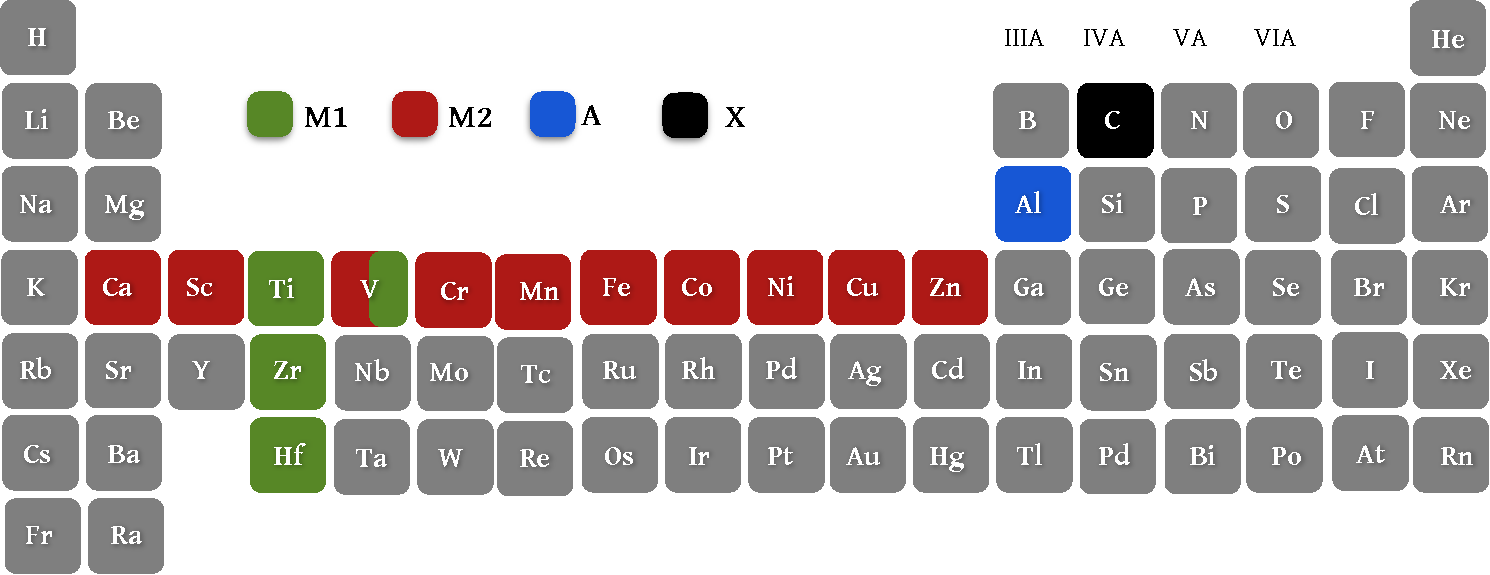
\includegraphics[width=0.95\textwidth]{figure_2}
\caption{Positions in the periodic table of elements used in this work}
\label{fig:SS_periodic_table}
\end{figure}

In this work, we use the MIT Ab-initio Phase Stability (MAPS)~\cite{van2002automating} code as implemented in the Alloy Theoretic Automated Toolkit (ATAT)~\cite{vanderwalleATAT} package to construct a cluster expansion from the result of first-principles calculations, of (M1$_x$,M2$_{1-x}$)$_2$AlC), M1 = Ti, V, Hf, Zr and M2 = Ca, Sc, V, Cr, Mn, Fe, Co, Ni, Cu, Zn where M1 and M2 can exchange places in the M site as shown in \fig{fig:SS_periodic_table}. Our choice of M1 is motivated by the intention of identifying trends as we move down the 4th group of the periodic table. For M2, we move along the 4th period, to study the effect of increasing occupancy of the d orbital. We restrict ourselves to the 211 configuration of the MAX phase. Effectively, we perform cluster expansion calculations for 41 MAX systems. 
% %------------------------------------------------------------------------------------------------------------------------------------%
\section{Results}
\label{sec:results} 

Cluster expansion calculations carried out on the 41 alloy systems showed that there exist three definite regimes in the solid solution behavior across the (M1)$_2$AlC - (M2)$_2$AlC composition range: i) weak ordering tendency with a low energy of formation (regime I), ii) phase separation (Regime II) and iii) strong ordering tendency with a high energy of formation (regime III). The classification criteria for the formation energy was chosen to be $\approx 75 ~ meV/atom$. Systems which showed a ground state with a formation energy less than  $75 ~ meV/atom$ relative to the pure end-members were designated as low; while those systems exhibiting a ground state with a formation energy greater than  $75 ~ meV/atom$ relative to the pure end-members were designated as high. It should be noted that these are ground states only relative to the end members, and are not the true ground states since we do not consider the relative stability of (M1,M2)$_2$AlC with respect to unary, binary, and other ternary compounds that 
may participate in equilibria of the system. To be precise, they are pseudo-ground states. However, in this work, we shall refer to them as ground states keeping in mind this caveat. \textcolor{red}{Additionally, the results presented are ground-state calculations and as such do not account for temperature or vibrational effects. This work is inteneded to be used as a tool to narrow down the solid - solution space, after which further computational techniques may be applied to account for temperature effects, vibrational contributions and the effect of competitive phases.}

In the next sub-sections, we discuss representative results for the three regimes. 

\subsection{Representative Results}
 Cluster expansion results are presented for three prototypical systems: i) Ti$_2$AlC - V$_2$AlC  (regime I), ii) Ti$_2$AlC - Mn$_2$AlC  (regime II), and iii) Ti$_2$AlC - Zn$_2$AlC  (regime III). The energy landscape is plotted with respect to the alloy configuration. The convex hull construction is shown, with the lower bound indicating the ground-states. The pair effective cluster interactions (ECIs) are also plotted as a function of cluster diameter (defined as the maximum distance between any two sites in the cluster). Ground states are identified and their crystal structure  is investigated. Density of states of the ground state relative to those of the end members are analyzed to gain insight into the stability of the ground states. The crystallographic data for all identified ground states is included in the appendix. To lend further insight into the energetics of these alloy systems, we also calculated the upper/lower critical solid solution temperature ($T_{UCSS}/T_{LCSS}$) which are defined at the critical temperature above/below which the components of a mixture are 
miscible. In the case of regimes I and III, $T_{UCSS}$ is applicable \textcolor{red}{and the selected composition is the structure with the most negative formation energy, (i.e. the most stable ground state)}. For Regime II, we calculate $T_{LCSS}$, choosing the 50-50 composition where we find the apex of the energy hull. The critical temperatures are calculated by approximating the formation energy  ($\Delta H_f$) as in \eq{eq:T_SS}. \textcolor{red}{Here the ($\Delta H_f$) refers to the formation energy of the particular composition w.r.t the end-members} and x is the amount of $M_1$, while (1-x) is the amount of $M_2$ in the relevant structure.

\begin{equation}
  \Delta H_f = RT(x\ln x + (1-x)\ln(1-x)) , 
  \label{eq:T_SS}
\end{equation}

To better understand the ground-state structures found in the systems under consideration, the electronic density of
states of the ground-state structures were also calculated and plotted. For the systems which do not show any ground states, we picked the structures corresponding to the ones for which the critical temperatures were calculated and analyzed their density of states (DOS).
In this section, since we focus on the Ti$_2$AlC - V$_2$AlC,  Ti$_2$AlC - Mn$_2$AlC, and  Ti$_2$AlC - Zn$_2$AlC alloy systems we only include the cluster expansions, ECIs, crystal structures and density of states relevant to these alloys. The detailed results for the remaining 39 alloy systems may be found in the appendix. 

%--------------------------------------------------------------------------------------------------------------------------------------------
\subsubsection{Regime I: Weak ordering}

\fig{fig:TiV} (a) shows the resulting ground state of the (Ti,V)$_2$AlC system indicated through the convex hull construction. 
Configuration space spanning structures with up to 48 atoms per primitive cell were explored. A clear tendency to order  at the (Ti$_{0.5}$V$_{0.5}$)$_2$AlC composition is seen. The formation energy of this ground-state is $\approx$ -8 meV/atom, which is not very significant. The solid line indicates the energy of equivalent random solutions, calculated using the following~\cite{liu2005structure}:
\begin{equation}
\frac{E_{random}}{N_{spins}} = \sum_{\alpha} J_{\alpha} m_{\alpha}\langle \sigma \rangle^{n_{\alpha}} 
\end{equation}
where the sum is over all the possible clusters $\alpha$, $m_{\alpha}$ is the multiplicity of the cluster, $n_{\alpha}$ is the number of sites in the cluster and $J_{\alpha}$ correspond to the ECIs. $\langle \sigma \rangle$ is the average spin concentration, related to the alloy concentration through $\langle \sigma \rangle = 2x-1$.

\fig{fig:TiV} (b) shows the convergence rate of the pair ECIs as a function of cluster diameter (atom-atom distance). It is seen that the pair ECIs converge rapidly as the cluster diameter increases. It is evident that the first-nearest-neighbor pair ECI dominates the energetics of the system which suggest an ordering tendency between Ti and V in the M sub-lattice as it is energetically favorable to have Ti-V pairs.
The crystal structure of the ground state is shown in \fig{fig:POSCAR_V}. It is seen that mixing in the M layer shows some amount of ordering. The $T_{UCSS}$ for this structure is calculated to be 112 K, which is very low. This low value attests to the observation that the identified ground state is not very stable and may easily decompose into a mixture of binary compounds when the effect of competing phases is included.

The  total DOS and the atom-projected  DOS  for the $Ti_2AlC$ MAX phase is shown in \fig{fig:TiV_end_members_DOS} a. The red color shows the contribution of the d band, the green region details the p band and the blue depicts the contribution of the s band. The structure is seen to be metallic, with the d-band contribution from Ti ions contributing the most to the conductivity. A pronounced trough at the fermi level points to the stability of the $Ti_2AlC$ MAX phase. By examining the atom-projected DOS, it is seen that the peaks centered around -−1 eV correspond to hybridized p-Al and d-Ti states while the peaks close to -−2.5 eV correspond to hybridized p-C and d-Ti states. 

\fig{fig:TiV_end_members_DOS} b describe the total DOS and the atom-projected  DOS  for the $V_2AlC$ MAX phase. The peaks in the upper part of the valence band at around --2 eV correspond to hybridized d-V, and p-Al states while the peak around --4 eV originates due to the hybridized s-Al, d-V and p-C states. The DOS at the fermi level originates from the 3d-V states and will contribute to electrical conductivity.

\fig{fig:TiV_DOS} show the total DOS and the atom-projected  DOS  for the (Ti$_{0.5}$V$_{0.5}$)$_2$AlC ground-state structure. The distinct trough at the fermi level indicates the stability of the phase. The peak at around -1.2 eV correspond to hybridized d-Ti, d-V, and p-Al states, which is shifted downward from those of $Ti_2AlC$ and upward from that of $V_2AlC$. The peak around --3.5 eV originates due to the hybridized s-Al, d-V, d-Ti and p-C states and is shifted downward from those of $Ti_2AlC$ and upward from that of $V_2AlC$. These low-lying states result in strong (Ti,V) - Al and (Ti,V)-C interactions.  \textcolor{red}{Also, a shallow shallow trough is seen at the fermi level, corresponding to the low formation energy (weak ordering) of Regime I.}

 \begin{figure}[!htb]
	\centering
	\subfigure [Ground state at 0 K.]{
	  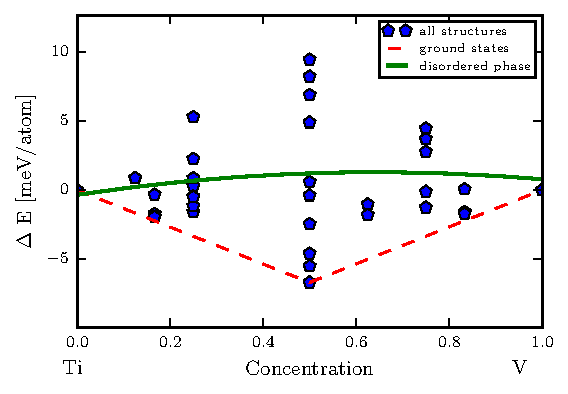
\includegraphics[width=0.55\textwidth]{figure_3a.pdf}}
	\subfigure[ECIs as a function of cluster diameter ]{
	  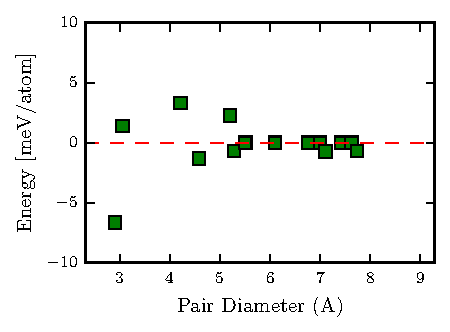
\includegraphics[width=0.4\textwidth]{figure_3b.pdf}}
	\caption{Cluster expansion for the $(Ti,V)_2AlC$ system.}	
	\label{fig:TiV}
\end{figure}

\begin{figure}[!htb]
\centering
\includegraphics[scale=0.7]{{figure_4.pdf}}
\caption{Crystal structure of (Ti$_{0.5}$V$_{0.5}$)$_2$AlC}
\label{fig:POSCAR_V}
\end{figure}

\begin{figure}[!htb]
\centering
\subfigure[ $Ti_2AlC$ ]{
  \includegraphics[width=0.45\textwidth]{{figure_5a.pdf}}}
  \hspace{1em}
\subfigure[ $V_2AlC$ ]{
  \includegraphics[width=0.45\textwidth]{{figure_5b.pdf}}}
\caption{Calculated electronic density of states (DOS) for a) $(Ti)_2AlC$ and b) $(V)_2AlC$ . Red, blue and green colors indicate the contributions of the d, s and p orbitals respectively. The top panels indicate the total and orbital projected density of states while the middle and lower panels indicate the site-projected density of states. }
\label{fig:TiV_end_members_DOS}
\end{figure}

\begin{figure}[!htb]
\centering
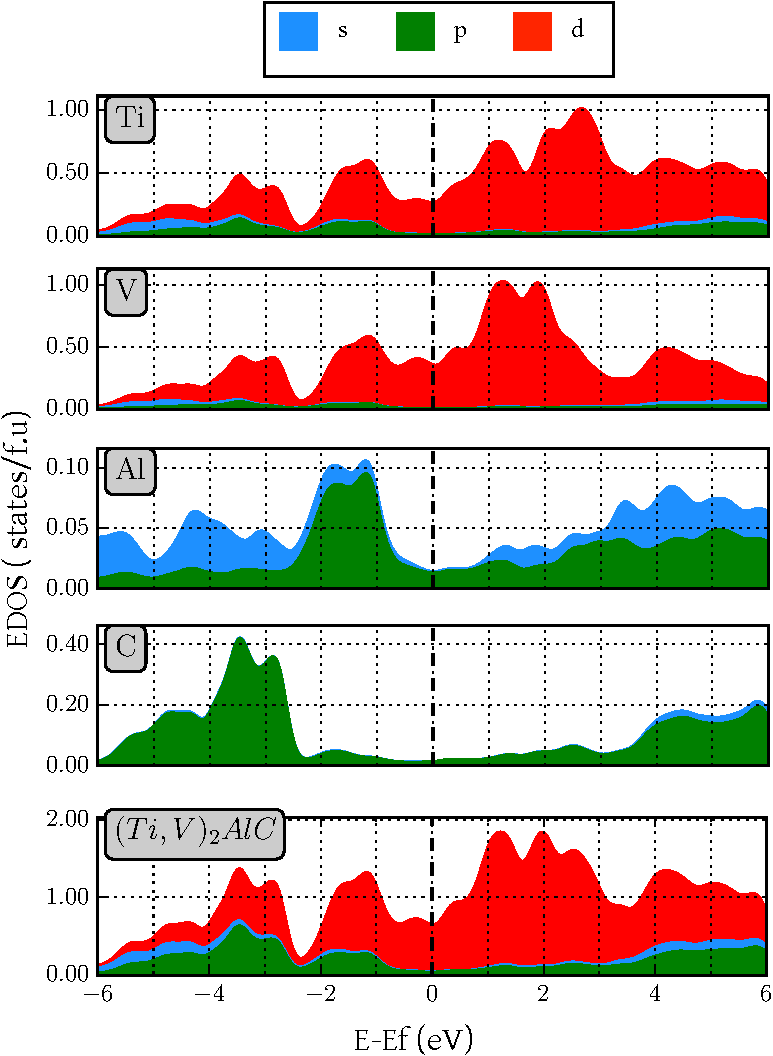
\includegraphics[width=0.45\textwidth]{figure_6.pdf}
\caption{Calculated electronic density of states (DOS) of (Ti$_{0.5}$V$_{0.5}$)$_2$AlC.Red, blue and green colors indicate the contributions of the d, s and p orbitals respectively. The top panel indicate the total and orbital projected density of states while the middle and lower panels indicate the site-projected density of states. }
\label{fig:TiV_DOS}
\end{figure}
%--------------------------------------------------------------------------------------------------------------------------------------------
\subsubsection{Regime II: Phase separation}

\fig{fig:TiMn} (a) shows the cluster expansion of the (Ti,Mn)$_2$AlC system. From the figure it is seen that all the identified structures have an energy higher than that of the end-members. It is important to bear in mind that the $Mn_2AlC$ MAX phase itself is not a stable MAX phase~\cite{mockute2013synthesis}. In this case, no ground-states are identified and contrary to the previous example, the system shows a tendency to phase separate rather than to order. A stable solid-solution is unlikely. \fig{fig:TiMn} (b) shows shows that the pair ECIs converge rapidly as the cluster diameter increases. 

The structure at the (Ti$_{0.5}$Mn$_{0.5}$)$_2$AlC composition with the lowest energy is selected to calculate the critical solid solution temperature which is found to be 370 K. The crystallographic details of this structure are shown in \fig{fig:POSCAR_Mn}. The $M_1$ and $M_2$ layers show no mixing and the Mn and Ti atoms fill separate layers, exhibiting sub-lattice separation. 

\fig{fig:TiMn_DOS} a describes the total DOS and the atom-projected  DOS  for the $Mn_2AlC$ MAX phase. The structure is seen to be metallic, with the d-band contribution from Mn ions contributing the most to the conductivity (at the Fermi level) as well as the valence band. The peaks in the upper part of the valence band at around -0.75 eV correspond to d-Mn states while the peak around -2.6 eV originates due to the hybridized p-Al, d-Mn states. Lower energy states around -4.5 eV appear due to the hybridization of d-Mn, s-Al and p-C states. 

\fig{fig:TiMn_DOS} b shows the total DOS and the atom-projected  DOS  for the (Ti$_{0.5}$Mn$_{0.5}$)$_2$AlC (pseudo) ground-state structure. The states at the Fermi level (i.e the absence of a trough like feature) indicate the instability of the phase. The first peak on the negative side of the fermi level is at around -1.3 eV due to hybridized d-Ti, d-Mn, and p-Al states and is shifted downward from the $Mn_2AlC$ peak and upward from the $Ti_2AlC$. Further low-energy peaks are observed at -2.3 eV (hybridized d-Mn, p-Al) and -4 eV (d-Mn and p-C) which are shifted upward from the $Mn_2AlC$ peak and downward from the $Ti_2AlC$ peak. \textcolor{red}{We see a peak in the vicinity of the fermi level corresponding to the positive formation energy (w.r.t the end members) which points to the tendency of the solid-solution to phase separate.} 


 \begin{figure}[!htb]
	\centering
	\subfigure [Ground state at 0 K.]{
	  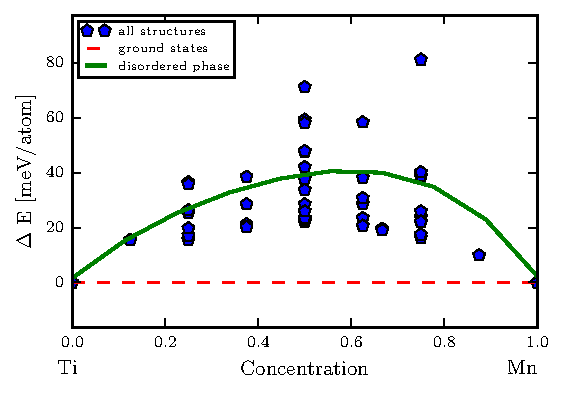
\includegraphics[width=0.55\textwidth]{figure_7a.pdf}}
	\subfigure[ECIs as a function of cluster diameter ]{
	  \includegraphics[width=0.4\textwidth]{{figure_7b.pdf}}}
	\caption{Cluster expansion for the $(Ti,Mn)_2AlC$ system.}	
	\label{fig:TiMn}
\end{figure}

\begin{figure}[!htb]
\centering
\includegraphics[scale=0.7]{{figure_8.pdf}}
\caption{Crystal structure of (Ti$_{0.5}$Mn$_{0.5}$)$_2$AlC}
\label{fig:POSCAR_Mn}
\end{figure}

\begin{figure}[!htb]
\centering
\subfigure[ $Mn_2AlC$ ]{
  \includegraphics[width=0.45\textwidth]{{figure_9a.pdf}}}
\subfigure[ (Ti$_{0.5}$Mn$_{0.5}$)$_2$AlC ]{
  \includegraphics[width=0.45\textwidth]{{figure_9b.pdf}}}
\caption{Calculated electronic density of states (DOS) for a)$(Mn)_2AlC$ and b) (Ti$_{0.5}$,V$_{0.5}$)$_2$AlC. Red, blue and green colors indicate the contributions of the d, s and p orbitals respectively. The top panels indicate the total and orbital projected density of states while the middle and lower panels indicate the site-projected density of states.}
\label{fig:TiMn_DOS}
\end{figure}

%--------------------------------------------------------------------------------------------------------------------------------------------
\subsubsection{Regime III: Strong ordering}

\fig{fig:TiZn} (a) shows the resulting ground state of the (Ti,Zn)$_2$AlC system indicated through the convex hull construction. 
The system is seen to favor ordering at the (Ti$_{1/3}$V$_{2/3}$)$_2$AlC composition. The formation energy of this ground-state is $\approx$ -104 meV/atom, which very high especially when compared to that of the (Ti,V)$_2$AlC system. The pair ECIs rapidly converge and the first-nearest-neighbor pair ECI dominates the energetics of the system as seen in \fig{fig:TiZn} (b). From this, again, we may expect to see  an ordering tendency between Ti and Zn in the M sub-lattice indicating that it is energetically favorable to have Ti-Zn pairs.
The crystal structure of the identified ground state is shown in \fig{fig:POSCAR_Zn}. It is seen that mixing in the M layer is ordered. The $T_{UCSS}$ for this structure is calculated to be 1616 K, which is very high, 8 times higher than that of (Ti,V). This indicates that the identified ground state is very stable and and the (Ti,Zn)$_2$AlC system may prove to have a stable solid-solution, without considering energetics of competitive phases.

\fig{fig:TiZn_DOS} a describes the total DOS and the atom-projected  DOS  for the $Zn_2AlC$ MAX phase.The DOS for $Zn_2AlC$ differs from the structures already examined in that we see continuous occupation over the entire valence band. 5 peaks are observed, ranging in energy from -0.5 eV to 5eV all originating due to hybridized d-Zn, s,p-Al and p-C states. 

\fig{fig:TiZn_DOS} b shows the total DOS and the atom-projected  DOS  for the (Ti$_{1/3}$Zn$_{2/3}$)$_2$AlC ground-state structure. A low-energy peak is observed on the negative side of the fermi level at around -2 eV due to hybridized d-Ti,Zn and p-C states and is shifted downward from the $Ti_2AlC$ and the $Ti_2AlC$ peaks. \textcolor{red}{There is a deep trough at the fermi level corresponding to the highly negative formation energy and high ordering tendencies of the compound typical of Regime III.} 

 \begin{figure}[!htb]
	\centering
	\subfigure [Ground state at 0 K.]{
	  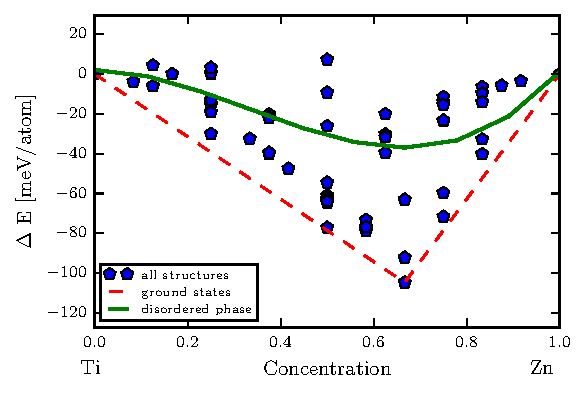
\includegraphics[width=0.55\textwidth]{figure_10a.pdf}}
	\subfigure[ECIs as a function of cluster diameter ]{
	  \includegraphics[width=0.4\textwidth]{{figure_10b.pdf}}}
	\caption{Cluster expansion for the $(Ti,Zn)_2AlC$ system.}	
	\label{fig:TiZn}
\end{figure}

\begin{figure}[!htb]
\centering
\includegraphics[scale=0.7]{{figure_11.pdf}}
\caption{Crystal structure of (Ti$_{1/3}$Zn$_{2/3}$)$_2$AlC}
\label{fig:POSCAR_Zn}
\end{figure}

\begin{figure}[!htb]
\centering
\subfigure[ $Zn_2AlC$ ]{
  \includegraphics[width=0.45\textwidth]{{figure_12a.pdf}}}
\subfigure[ Ti$_{0.5}$Zn$_{0.5}$)$_2$AlC ]{
  \includegraphics[width=0.45\textwidth]{{figure_12b.pdf}}}
\caption{Calculated electronic density of states (DOS) for a)$(Zn)_2AlC$ and b) (Ti$_{0.5}$,V$_{0.5}$)$_2$AlC. Red, blue and green colors indicate the contributions of the d, s and p orbitals respectively. The top panels indicate the total and orbital projected density of states while the middle and lower panels indicate the site-projected density of states.}
\label{fig:TiZn_DOS}
\end{figure}
%--------------------------------------------------------------------------------------------------------------------------------------------
\subsection{Overall Description of Results}
\fig{fig:MAX_overall_results_energies} presents a summary of the cluster expansion results for all 41 systems considered depicting the three observed regimes i) ordering tendency with a low energy of formation (Regime I-yellow), ii) phase separation (Regime II-orange) and iii) ordering tendency with a high energy of formation (Regime III-blue). The corresponding critical solid-solution temperatures $T_{UCSS}/T_{LCSS}$ are also indicated. As expected, the critical temperatures for Regimes I and II are calculated to be a few hundred K, while most of the compounds in Regime III have disordering temperatures above $1,000$ K. The higher the temperature, the greater the stability of ordered or phase separation states. Temperatures within a few hundred Kelvin, on the other hand, suggest that solid solutions are likely to be observed. It should be noted that in this analysis, the critical temperatures are used purely as a measure of relative stability and are approximations.  It is seen that of the 41 cases, 11 alloy systems fall within Regime I, 18 in Regime II and 12 in Regime III. The formation energies for the lowest energy ground states are indicated in \fig{fig:MAX_overall_results_energies}. As mentioned earlier, systems which showed a ground state with a formation energy less (in magnitude) than  75 meV/atom relative to the pure end-members were designated as low; while those systems exhibiting a ground state with a formation energy greater than  75 meV/atom relative to the pure end-members were designated as high.

Based on the cluster expansion calculations, without considering the effect of competitive phases, the 11 regime I systems have a very low probability of forming a stable solid solution. It is possible that once the effect of the competing binary phases is accounted for, the identified ordered phases will decompose into more stable binary compounds. However, as mentioned earlier, the (Ti,V)$_2$AlC system, which belongs to regime I, (Ti,V)AlC has been shown to have complete solute solubility experimentally \cite{schuster1980ternary,meng2005strengthening,yeh2014combustion}. Thus for regime I systems, stable solid solution may or may not be possible.  In the case of the 18 Regime II systems, there are no stable ordered phases even when the effect of competing phases is neglected. A few systems within Regimes I and II---those for whose critical solid-solution temperatures are within a few hundred K---are likely to form at least metastable solid solutions. Unfortunately, this ignores the competition with other phases in the ground state of the corresponding quaternary system. If both end members have been synthesized (and are thus likely to be at least metastable), compounds within Regime I are likely to have at least some degree of solubility for each other due to the stabilizing effect of configurational entropy. Compounds in Regime II that have disordering temperatures are within a few hundred Kelvin and in which both end members are stable are also likely to have some degree of solubility, at least at elevated temperatures. Compounds within Regime III, on the other hand, are so stable that some of them may likely compete successfully against the ground state in the system. Moreover, some of these systems may decompose into solid solutions at technologically relevant temperatures. 


\begin{figure}[!htb]
\centering
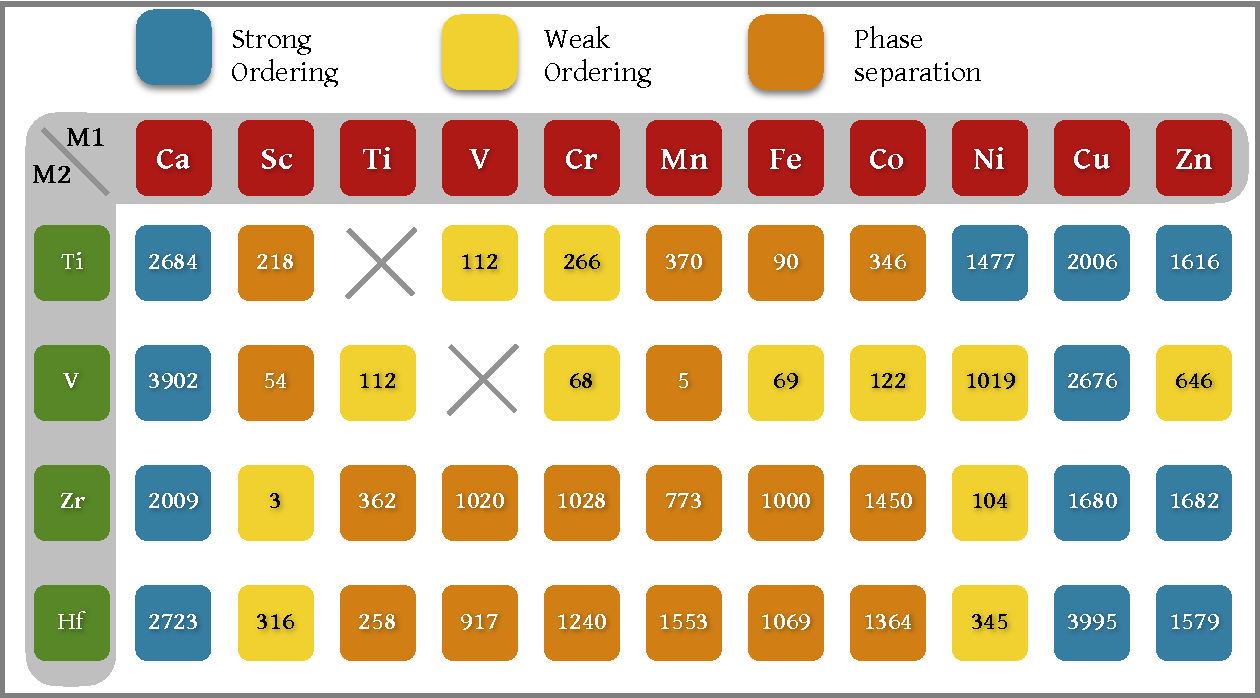
\includegraphics[width=0.95\textwidth]{figure_13.pdf}
\caption{Summary of the Cluster expansion  results showing the three regimes i) Regime I (yellow) , ii) Regime II (yellow) and iii) Regime III (blue) and the critical temperatures $T_{UCSS}/T_{LCSS}$}
\label{fig:MAX_overall_results}
\end{figure}

\begin{figure}[!htb]
\centering
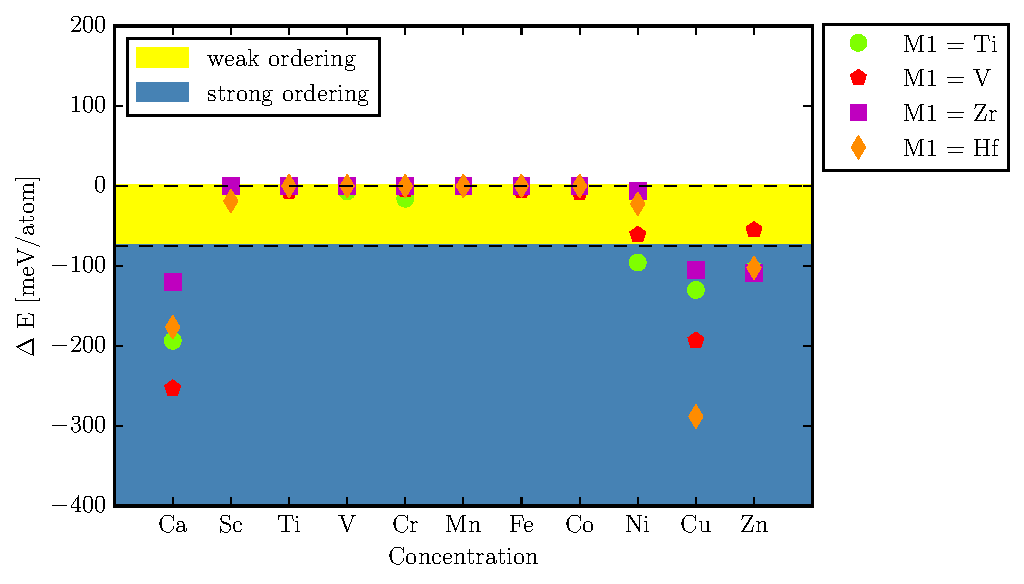
\includegraphics[scale=0.95]{figure_14.pdf}
\caption{Formation energies of ground states}
\label{fig:MAX_overall_results_energies}
\end{figure}
% %------------------------------------------------------------------------------------------------------------------------------------%
\section{Discussion}
\label{sec:discussion}

From \fig{fig:MAX_overall_results_energies} it is seen that the low formation energy and phase separating systems ( yellow and orange) are clustered towards the middle of the periodic table, while the high formation energy systems are predominantly found towards the ends (with the exception of the (Zr,V)$_2$AlC system). Of these, Calcium is an alkaline earth metal while the rest are transition elements. If we keep aside calcium, then it is worthwhile to view the results from the perspective of the number of d electrons. As we move from left to right, the number of d electrons increases from one for scandium to 10 for zinc. Thus, it would appear, that almost filled or fully filled d-bands are a feature of  regime III systems, while semi-filled d-bands characterize regime I \& II.

The Hume-Rothery rules~\cite{hume1934freezing} for  substitutional solubility indicate that a metal will dissolve a metal of higher valency to a greater extent than one of lower valency. The solute and solvent atoms should typically have the same valence in order to achieve maximum solubility. Of the elements under consideration, Ti, Hf,Zr, Mn and Co have valency of 4. All the $M_1$-$M_2$ combinations arising from these 5 elements ( Ti-Mn, Ti-Co, Hf-Mn, Hf-Co, Zr-Mn, Zr-Co) however, show a tendency to phase separate. Since Ti, Zr, and Hf do not show similar trends in spite of having the same valence and number of d-electrons, these features yield no insight. Electronegativity increases as we move from left to right along the 4th row and decreases as we move down along the 4B period. For maximum solubility, the solute and solvent should have similar electronegativity. The electronegativity difference was calculated for the $M_1$-$M_2$ pairs but could not be related to the trends observed. 

Atomic size difference is another feature which was explored. The Hume-Rothery rules indicate that substitutional solid solution occurs only if the relative difference between the atomic diameters (radii) of the two species is
less than 15\%. This criteria, again, is ineffective here since all the transition elements have very similar atomic diameters. The \% difference between the metallic radii was also calculated for the $M_1$-$M_2$ pairs, however no correlation was found between the difference in metallic radii and the cluster expansion behavior of the pairs.
 
Orbital radii such as the Waber-Cromer radii~\cite{waber1965orbital} and the Zunger~\cite{zunger1980systematization} radii based on model pseudopotential fits  and their linear combinations have long been used to extract structural, chemical and stability trends~\cite{bloch1972structural}. Building upon the valence bond theory of solids proposed by Pauling~\cite{pauling1932nature}, it has been theorized by Bloch\etal~\cite{bloch1972structural} that functional linear combinations~\cite{chelikowsky1978quantum} of the s and p orbitals may be used to classify AB compound interactions, where $r_{\sigma}$ and $r_{\pi}$ are given by:

\begin{equation}
r_{\sigma} = ({r_s}^A +{r_p}^A) - ({r_s}^B +{r_p}^B) 
\end{equation}
\begin{equation}
r_{\pi} = ({r_s}^A -{r_p}^A) + ({r_s}^B -{r_p}^B)
\end{equation}

\noindent $r_{\sigma}$ delineates the effect of electronegativity difference between A- and B-atoms, while $r_{\pi}$ quantifies  the directional nature of bonding through hybridization between s- and p-orbitals of A- and B-atoms. \textcolor{red}{${r_s}^A$  and ${r_p}^A$ denote the s-orbital and p-orbital radii for element A and  ${r_s}^B$  and ${r_p}^B$ denote the s-orbital and p-orbital radii for element B.}
In this work, we used both the Waber-Cromer and Zunger orbital radii in an effort to explain the observed trends. In line with the recent work by Lookman \etal~\cite{balachandran2016adaptive}, we used s, p and d orbital radii for $M_1$ and $M_2$, and s-p orbital radii for A and X elements. A priori, attempts to find classifiers using these linear combinations of orbital radii for the $M_1$-$M-2$ , ($M_1$,$M_2$)-A, ($M_1$,$M_2$)-X pairs were unsuccessful.
Of these, \fig{fig:orbital_radii} (a) shows the $r_{\sigma}$ Vs $r_{\pi}$ plot using the Zunger radii. These are non-weighted absolute values.
No distinct correlation is observed,  the systems belonging to regime I and III ( red, green and blue show a slight tendency to cluster.
Posteriori analysis of the relationship between composition weighted $r_{\sigma}$ and $r_{\pi}$  using the Zunger radii of the  regime I \& III $M_1$-$M_2$ pairs for the identified ordered structures yielded interesting results as shown in \fig{fig:orbital_radii} (b). Here, definite clustering is seen with the regimes I \& III, with the clustering of systems of similar composition. This is not a definitive or robust classification however, since by weighting we are biasing the classification. A non-weighted uniform distribution when weighted will realistically show clustering which is an artifact of the weighting process and not a correlation.

 \begin{figure}[!htb]
	\centering
	\subfigure [$r_{\sigma}$ Vs $r_{\pi}$ (Not Weighted)]{
	  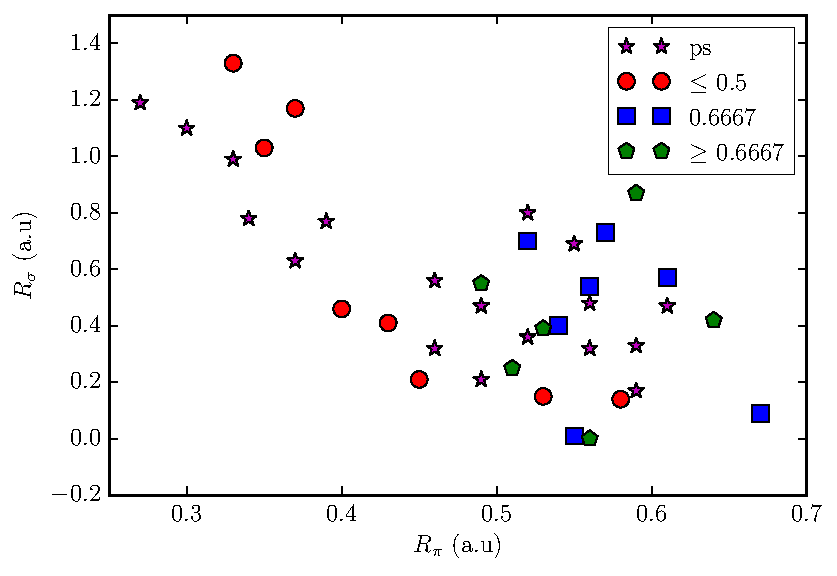
\includegraphics[width=0.48\textwidth]{figure_15a.pdf}}
	\subfigure[$r_{\sigma}$ Vs $r_{\pi}$ (Weighted) ]{
	  \includegraphics[width=0.48\textwidth]{{figure_15b.pdf}}}
	\caption{Orbital radii (Zunger) relationships: (a) Average radii (b) Weighted average radii }	
	\label{fig:orbital_radii}
\end{figure}

However, it is worth noting that the lack of success in isolating a physical basis for the observed trends is indicative of the complex forces at work in the thermodynamics of these systems. All the features, or a combination of them or none of them may be contributing to the phase-selection in these quaternary systems. This validates our initial proposition that cluster expansion is an effective technique to identify the elements which are more likely to form solid solutions.

The results presented in the previous section show that for M$_1$ = Ti, (Ti,V)$_2$AlC and (Ti,Cr)$_2$AlC may form stable solid solutions. As mentioned earlier in Section \ref{sec:prior}, (Ti,V)$_2$AlC solid solutions have been synthesized and are known to exist~\cite{schuster1980ternary,meng2005strengthening,yeh2014combustion}. Solid solutions belonging to the (Ti,Cr)$_2$AlC have been identified by a number of independent researchers~\cite{schuster1980ternary}. For  M$_1$ = V, regime I systems include (V,M$_2$)$_2$AlC, with $M_2$ = Cr, Fe, Co,Ni, and Zn. Of these, (V,Cr)$_2$AlC has been synthesized~\cite{schuster1980ternary, barsoum2002thermal}. 

For M$_1$ = Zr, solid solutions may be possible with $M_2$ = Sc, and Ni. However, no previous work has been carried out on these alloys with the exception of recent work by Horlait\etal~\cite{horlait2016attempts}, wherein they attempted to fabricate (Zr,Ti)$_2$AlC solid-solution unsuccessfully. With M$_1$ = Hf, Regime I possibilities include $M_2$ = Sc, and 
Ni neither of which have been studied to date. Of the Regime II systems listed in \ref{fig:MAX_overall_results_energies}, Horlait \etal~\cite{horlait2016attempts} also attempted to synthesize (Zr,Cr)$_2$AlC but were unsuccessful. To the best knowledge of the authors, none of the Regime II systems have been synthesized. 


\subsection{The Problem of Phase Competition}

Cluster expansion calculations have been carried out explore the pseudo-binary region of the $(M_1)_2$AlC - $(M_2)_2$AlC composition space. While it is certainly useful as a first step in the exploration of the solid -solution configuration space, it is neither exhaustive nor complete. The topology of the binary $M_1$-$M_2$ phase space plays an important role in the stability of the system as more intermetallic binary phases will likely lead to a more complicated MAX solid solution phase space. Monte-Carlo methods may be applied to the cluster expansion results to generate a metastable phase diagram. However, to gain a true description of the energetics and stability of these systems it is necessary to include the effect of competing phases and construct a complete phase diagram. Cluster expansion may be used to identify the Regime II systems which are highly unlikely to form solid-solutions which may then be disregarded. Regime I systems are likely to form solid solutions, however because of the low formation energies the 
effect of competing binary and ternary phases is very important. These solid solutions may achieve stability and exist in combination with other phases. Similarly, Regime III systems, whose ground-states have higher formation energies are more likely to form solid-solutions. However, even in these cases, it is not possible to definitely evaluate the likelihood without considering the effect of competing phases. Dahlqvist \etal~\cite{dahlqvist2010stability}  put forward a model to predict the stability of undiscovered potential phases. They investigated the phase stability of M$n+1$AX$_n$ phases using DFT calculations in combination with
linear optimization procedures using the formation enthalpies of all known competing phases and were able to  completely reproduce experimental occurrences of stable MAX phases. 

\begin{table}[tbp!]
\centering
\setlength{\tabcolsep}{0.2cm}
\setlength\extrarowheight{2.5pt}
\begin{tabular}{llc}
\hline \hline
Competing  Phases                   & Amount                 & $\Delta H_f$ (eV) \\
\hline 
TiC                    & 0.54                   & -0.42552                  \\
Al$_4$C$_3$                  & 0.15                   & -0.0147                   \\
TiAl$_3$                  & 0.13                   & -0.05252                  \\
Zn                     & 1.33                   & 0                         \\
\hline
\multicolumn{2}{l}{$\Delta H_f$} & -0.49274        \\
\hline \hline
\end{tabular}
\caption{Phase competition analysis for (Ti$_{0.33}$Zn$_0.66$)$_2$AlC. Listed are the possible resultant phases from phase decomposition of ordered structure obtained from the Open Quantum Materials Database~\cite{saal2013materials}. Energies listed are in eV/unit cell}
\label{tab:OQMD_TiZn}
\end{table}

For the prototypical Regime III scenario in (Ti,Zn)$_2$AlC, we explore the energetics of competing phases at 0 K for the ordered phase (Ti$_{0.33}$Zn$_0.66$)$_2$AlC. The Grand Canonical Linear Programming (GCLP)~\cite{r2007first,kirklin2013high} module of the Open Quantum Materials Database (OQMD)~\cite{saal2013materials} was used to determine the compositions of the possible phases if the ordered phase decomposes. The \textcolor{red}{possible} decomposition reaction is given by:
\begin{equation}
(Ti_{0.333}Zn_{0.667})_2AlC \rightarrow 0.15 Al_4C_3 + 0.54 TiC + 1.33 Zn + 0.13 TiAl_3
\end{equation}

The results are shown in Table \ref{tab:OQMD_TiZn}. We see that (Ti$_{0.33}$Zn$_0.66$)$_2$AlC may \textcolor{red}{chemically} decompose into a combination of TiC, TiAl$_3$, Al$4$C$_3$ and pure Zn. The formation energy of Ti$_{0.33}$Zn$_0.66$)$_2$AlC with respect to the Ti-Zn-Al-C phase space is -0.29 eV/atom while that of the decomposed phases sums to -0.49274 eV/unit cell which is -0.123 eV/atom. The difference in formation energies of (Ti$_{0.33}$Zn$_0.66$)$_2$AlC and the sum of the decomposed phases is -0.167 eV/atom, which indicates that at 0 K, the ordered phase is  \textcolor{red}{stable} and will not decompose,  \textcolor{red}{i.e. the decomposition reaction is thermodynamically improbable}. 
It is however also necessary to include the effect of finite temperature to get a complete picture of the stability energetics. For the Regime III systems it is worthwhile to explore the effect of competing phases at finite temperatures and calculate the complete phase diagram to evaluate the possibility of solid-solution formation, which will be explored in future works by the present authors. 
%------------------------------------------------------------------------------------------------------------------------------------%
\section{Conclusions}
\label{sec:conclusion}
Cluster expansion calculations were carried out at 0 K to study the effect of M site alloying on the solid solution behavior of 41 (M1,M2)$_2$AlC systems. Three regimes of behavior were observed, with 11 combinations (Regime I) showing weak ordering tendency, 18 (Regime II) systems showing a tendency to phases separate and 12  of them  (Regime III) showing strong ordering behavior. The stable and unstable ordered structures of three prototypical systems, were identified and their crystal structure and electronic density of states were analyzed. Of these, it was shown that Regime I \& Regime III have a greater likelihood of forming stable solid-solutions while the Regime II materials were identified as uncertain candidates. Consequently, a phase competition analysis was carried out for the regime III prototypical system (Ti,Zn)$_2$AlC and it was seen that taking into account the competing phases, the (Ti$_{0.33}$Zn$_0.66$)$_2$AlC ordered phase is the ground state at 0 K. 

Overall, phase separating systems were clustered toward the center of the periodic table with the tendency to ordering increasing as one moved outwards. Various features were then identified and calculated for all the  $M_1$-$M_2$ pairs in an effort to explain this trend. Of the 12 Regime III systems, disregarding the cases of $M_2$ = Ca, we found 8 systems which warrant a deeper study and may prove to be viable candidates for stable MAX solid-solutions. These systems will be analyzed taking into consideration the effect of phase competition and finite temperature properties and their phase diagrams will be constructed in future work by the authors with the final goal of furnishing the best candidates for new solid-solution MAX phases.
%------------------------------------------------------------------------------------------------------------------------------------%
\section{Acknowledgments}
\label{sec:ack}
We acknowledge support from NSF through Grants No. DMR-1410983 and CMMI-0953984. First-principles calculations by R.A., T.D and A.T. were carried out at the Texas A\& M Supercomputing Facility at Texas A\&M University as well as the Texas Advanced Computing Center (TACC) at the University of Texas at Austin. Preparation of the input files and analysis of the data have been performed using AFLOW~\cite{curtarolo2012aflowlib} and OQMD~\cite{saal2013materials}. The Texas A\&M Materials Modeling Automation Library (tammal) developed by R.A., A.T. and collaborators (soon to be released to the general scientific community) was used to carry out the HT cluster expansion calculations. The ATAT package~\cite{vanderwalleATAT} was used to carry out the cluster expansions. 

\bibliography{maxphases_cluster}

\end{document}
%------------------------------------------------------------------------------------------------------------------------------------%